\abouteditors

\vspace{-2cm}
\begin{center}

\includegraphics[width=.3\textwidth]{Photos/minku.jpg}
\end{center}

Dr. Leandro L. Minku is an Associate Professor at the School of Computer Science, University of Birmingham (UK). Prior to that, he was a Lecturer in Computer Science at the University of Leicester (UK). He received the PhD degree in Computer Science from the University of Birmingham (UK) in 2010. Dr. Minku's main research interests are machine learning in non-stationary environments / data stream mining, online class imbalance learning, ensembles of learning machines and computational intelligence for software engineering. His work has been published in internationally renowned journals such as IEEE Transactions on Neural Networks and Learning Systems, IEEE Transactions on Knowledge and Data Engineering, IEEE Transactions on Software Engineering and ACM Transactions on Software Engineering and Methodology. Among other roles, Dr. Minku is Associate Editor-in-Chief for Neurocomputing, Senior Editor for IEEE Transactions on Neural Networks and Learning Systems, and Associate Editor for Empirical Software Engineering Journal and Journal of Systems and Software. He was also the General Chair for the International Conference on Predictive Models and Data Analytics in Software Engineering (PROMISE 2019 and 2020), and Co-chair for the Artifacts Evaluation Track of the International Conference on Software Engineering (ICSE 2020).

\newpage
\

\vspace{3cm}
\begin{center}

\includegraphics[width=.3\textwidth]{Photos/cabral.jpg}
\end{center}

Dr. George Cabral received his PhD degree from the Federal University of Pernambuco (Brazil) in 2014. His postdoc was conducted at the University of Birmingham (UK) in 2019. Currently, he is an adjunct professor at the Department of Computing at the Federal Rural University of Pernambuco (Brazil). He serves as reviewer for reputed journals such as Neurocomputing and Applied Software Computing. In addition, he has systematically served as committee member in prestigious conferences such as ICSE, ASE and ICONIP. His recent plublications include papers in reputed venues such as IEEE Transactions on Software Engineering and at the International Conference on Software Engineering (ICSE). He has taught courses involving Computational Intelligence for more than a decade and since 2020 he is applying this knowledge in practice for auditing public finances at the state of Pernambuco - Brazil. His research interests include Novelty Detection, One-class Classification, Data Mining, Class Imbalance Learning, Software Defect Prediction, Concept Drift, Online Learning, etc.

\newpage

\

\vspace{3cm}
\begin{center}
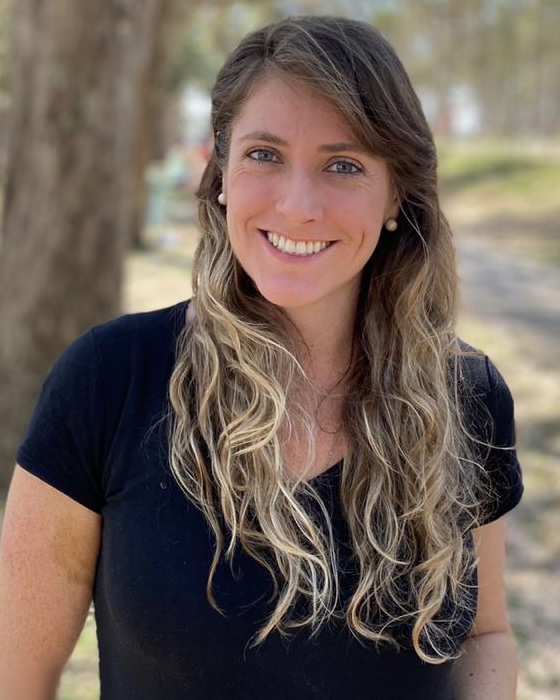
\includegraphics[width=.3\textwidth]{Photos/mar2022.jpg}
\end{center}

Marcella Scoczynski is an Assistant Professor at Federal University of Technology - Parana UTFPR, Brazil. She has done her PhD on Computer Engineering at Federal University of Technology - Parana UTFPR, Brazil. Her thesis has awarded at the Theses Competition during Brazilian Conference on Intelligent Systems (BRACIS 2018) and at the Theses Contest during 5th IEEE Latin American Conference on Computational Intelligence (LA-CCI 2018). Her main research interests are numerical and combinatorial optimization, evolutionary computation and metaheuristics (with a particular interest in estimation of distribution algorithms), and landscape analysis. She is a researcher in projects conducted by Frontier Development Lab (FDL), NASA and SETI Institute. 

\newpage
\

\vspace{3cm}
\begin{center}
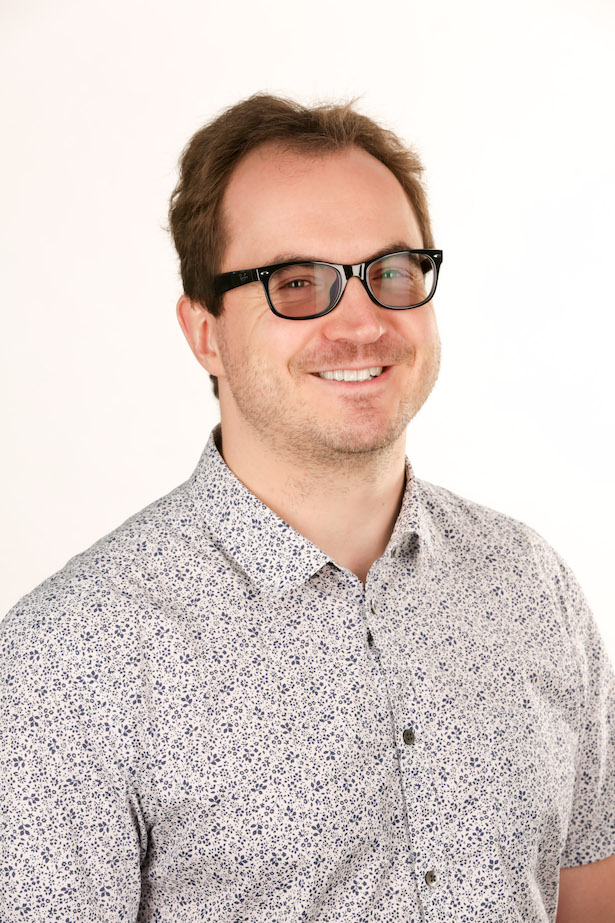
\includegraphics[width=.3\textwidth]{Photos/wagner.jpg}
\end{center}

Dr. Markus Wagner is an Associate Professor at Faculty of Information Technology, Monash University (Australia). He has done his PhD studies at the Max Planck Institute for Informatics in Saarbruecken, Germany and at the University of Adelaide, Australia. For the outcomes of his studies, he has received the university's Doctoral Research Medal --- the first for his school --- and three best paper awards. His research topics range from mathematical runtime analysis of heuristic optimisation algorithms and theory-guided algorithm design to applications of heuristic methods to renewable energy production, professional team cycling and software engineering. So far, he has been a program committee member 80+ times, and he has written 150+ articles with 200+ different co-authors. He has chaired several education-related committees within the IEEE CIS, where he also served as founding chair of two task forces. Markus is an ACM Lifetime Member, is on SIGEVO's Executive Board and serves as the first ever Sustainability Officer. He has contributed to GECCOs as Workshop Chair and Competition Chair, and most recently as General Chair.

